% ---------------------------------------------------------------------------
% fig:fliparch -- the LAT EEG encoder, laid out for \small type.
% ---------------------------------------------------------------------------
\begin{tikzpicture}[x=1cm,y=1cm]

\tikzset{
  ptitle/.style ={font=\normalsize\bfseries, text=inkgray, anchor=north west,
                  inner sep=0pt},
  note/.style   ={font=\scriptsize, text=inkgray!80, inner sep=1.5pt},
  op/.style     ={circle, draw=inkgray!80, fill=white, line width=0.7pt,
                  inner sep=0pt, minimum size=10pt, font=\scriptsize},
  stem/.style   ={line width=0.85pt, draw=eegblue},
  sgn/.style    ={font=\scriptsize, text=inkgray!80, inner sep=0.6pt},
  jdot/.style   ={circle, fill=eegblue, inner sep=0pt, minimum size=2.6pt},
  hop/.style    ={},
  shot/.style   ={inner sep=0pt, draw=inkgray!45, line width=0.6pt},
}
% token grid, from the top-left: #1 cols, #2 rows, #3 cell w, #4 cell h, #5 fill
\newcommand{\tokgrid}[5]{%
  \foreach \ti in {1,...,#1}{\foreach \tj in {1,...,#2}{
     \fill[#5, draw=eegblue!45, line width=0.25pt]
       ({(\ti-1)*#3},{-(\tj-1)*#4}) rectangle ({\ti*#3-0.018},{-\tj*#4+0.018});}}}

% =========================== panel grounds ================================
\path[panel] (-0.12,6.68) rectangle (13.52,9.64);   % (a)
\path[panel] (-0.12,2.19) rectangle ( 6.55,6.53);   % (b) gate + flip
\path[panel] ( 6.75,2.19) rectangle (13.52,6.53);   % (c) criss-cross
\path[panel] (-0.12,-0.93) rectangle ( 6.85,1.98);  % (d)
\path[panel] ( 7.10,-0.93) rectangle (13.52,1.98);  % (e)

\begin{scope}[yshift=-1.80cm]
% ===================== (a) tokenizing the EEG =============================
\node[ptitle] at (0.16,11.26) {(a) EEG tokenization};

\node[lbl, anchor=south west] at (0.34,10.52) {$\mathbf{X}_t\in\mathbb{R}^{C\times T}$};
\begin{scope}[shift={(0.34,10.32)}] \eegtrace{2.60}{1.00}{6}{eegblue} \end{scope}
\foreach \k in {0,...,5}{
  \draw[inkgray!35, line width=0.5pt, dash pattern=on 1.3pt off 1.3pt]
    ({0.34+\k*0.52},9.32) -- ({0.34+\k*0.52},10.38);}
% a patch is a time slice WITHIN one channel, not a column across channels
\draw[fill=eegblue, draw=eegblue!70, line width=0.5pt, opacity=0.30,
      rounded corners=1pt] (0.86,9.40) rectangle (1.38,9.58);
\draw[inkgray!55, line width=0.5pt] (1.12,9.38) -- (1.12,9.22);
\node[lbl, anchor=north] at (1.32,9.20) {one patch, one channel};
\node[lbl, anchor=north] at (1.45,8.92) {$C$ channels, $T$ samples};

\draw[eflow] (3.06,10.00) -- (3.46,10.00);
\draw[stem] (3.56,10.44) -- (3.56,9.56);
\draw[eflow] (3.56,10.44) -- (4.06,10.44);
\draw[eflow] (3.56,9.56) -- (4.06,9.56);
\node[mod, minimum width=1.90cm, minimum height=0.54cm] (fta) at (5.05,10.44) {waveform};
\node[mod, minimum width=1.90cm, minimum height=0.54cm] (ftb) at (5.05,9.56) {spectral};
\node[lbl, align=center] at (5.05,10.00) {$f_{\mathrm{emb}}$};
\node[tag, anchor=north] at (5.05,9.12) {patch embedding};
\node[op] (aplus) at (6.55,10.00) {$+$};
\draw[eflow] (fta.east) -- (aplus.north west);
\draw[eflow] (ftb.east) -- (aplus.south west);
\draw[eflow] (aplus.east) -- (7.10,10.00);

\begin{scope}[shift={(7.16,10.72)}] \tokgrid{5}{6}{0.30}{0.26}{eeglight} \end{scope}
\node[lbl, anchor=south] at (7.91,10.88)
     {$\mathbf{Z}\in\mathbb{R}^{C\times N\times D_e}$ --- EEG tokens};
\draw[{Stealth[length=1.6mm,width=1.2mm]}-{Stealth[length=1.6mm,width=1.2mm]},
      inkgray!60, line width=0.5pt] (8.86,10.68) -- (8.86,9.20);
\node[lbl, anchor=west] at (8.96,10.00) {$C$};
\draw[{Stealth[length=1.6mm,width=1.2mm]}-{Stealth[length=1.6mm,width=1.2mm]},
      inkgray!60, line width=0.5pt] (7.16,9.00) -- (8.62,9.00);
\node[lbl, anchor=north] at (7.89,8.94) {$N$};
\node[lbl, anchor=west, align=left] at (9.45,10.00)
     {$D_e$ features\\per token};

% ===================== (b) the learned gate, then the flip ================
% The gate acts on the patch embedding, before any Transformer block, so it
% comes before (c) in the pipeline as well as on the page.
\begin{scope}[xshift=-6.72cm, yshift=-0.16cm]
% ===================== (b) the gate and the flip ==========================
\node[ptitle] at (6.91,8.31) {(b) Learned gate $\mathbf{G}$ and flip $\mathcal{P}$};

\node[lbl, anchor=south west] at (6.91,7.62) {$\mathbf{Z}$ --- as recorded};
\foreach \y/\nm in {7.42/C3, 7.02/C4, 6.62/Cz}{
  \node[lbl, anchor=east] at (7.08,\y) {\nm};
  \draw[fill=eeglight, draw=eegblue!60, line width=0.4pt, rounded corners=0.8pt]
    (7.14,{\y-0.12}) rectangle (7.56,{\y+0.12});}
\foreach \y in {7.42,7.02,6.62}{\draw[stem] (7.56,\y) -- (7.66,\y);}
\draw[stem] (7.66,7.42) -- (7.66,6.62);
\draw[eflow] (7.66,7.02) -- (8.01,7.02);
\node[mod, minimum width=1.30cm, minimum height=0.56cm] (gate) at (8.70,7.02)
     {$\mathbf{G}=\sigma(\cdot)$};
\draw[eflow] (9.39,7.02) -- (9.74,7.02);
\draw[stem] (9.74,7.42) -- (9.74,6.62);
\foreach \y in {7.42,7.02,6.62}{\draw[stem] (9.74,\y) -- (9.88,\y);}

\foreach \y in {7.42,7.02,6.62}{
  \draw[fill=bilight, draw=bislate, line width=0.45pt] (9.90,\y) rectangle ++(0.46,0.16);
  \draw[fill=latlight, draw=latred, line width=0.45pt] (9.90,{\y-0.16}) rectangle ++(0.46,0.16);}
\foreach \y in {7.42,7.02,6.62}{
  \draw[-{Stealth[length=1.8mm,width=1.3mm]}, bislate, line width=0.9pt]
    (10.40,{\y+0.08}) -- (11.86,{\y+0.08});}
\draw[-{Stealth[length=1.8mm,width=1.3mm]}, latred, line width=0.9pt]
  (10.40,7.34) -- (11.86,6.94);
\draw[-{Stealth[length=1.8mm,width=1.3mm]}, latred, line width=0.9pt]
  (10.40,6.94) -- (11.86,7.34);
\draw[-{Stealth[length=1.8mm,width=1.3mm]}, latred, line width=0.9pt]
  (10.40,6.54) -- (11.86,6.54);
\foreach \y in {7.42,7.02,6.62}{
  \draw[fill=bilight, draw=bislate, line width=0.45pt] (11.92,\y) rectangle ++(0.46,0.16);
  \draw[fill=latlight, draw=latred, line width=0.45pt] (11.92,{\y-0.16}) rectangle ++(0.46,0.16);}
\node[lbl, anchor=south, align=center] at (12.15,7.62)
     {$\mathcal{P}(\mathbf{Z})$\\flipped};
\node[anchor=west] at (12.20,7.22) {};

\begin{scope}[shift={(7.85,6.02)}]
  \headtop{0.44}{eeglight}{eeglight}
  \foreach \x/\y in {-0.26/0.00, 0.26/0.00, -0.19/0.23, 0.19/0.23,
                     -0.17/-0.22, 0.17/-0.22}{
    \draw[fill=latred!70, draw=latred, line width=0.35pt] (\x,\y) circle (0.048);}
  \draw[fill=bislate!70, draw=bislate, line width=0.35pt] (0,0) circle (0.046);
  \foreach \xa/\xb/\yy/\bd in {-0.26/0.26/0.00/40, -0.19/0.19/0.23/32}{
    \draw[latred!85, line width=0.6pt,
          {Stealth[length=1.4mm,width=1.1mm]}-{Stealth[length=1.4mm,width=1.1mm]}]
      (\xa,\yy) to[bend left=\bd] (\xb,\yy);}
  \draw[latred!85, line width=0.6pt,
        {Stealth[length=1.4mm,width=1.1mm]}-{Stealth[length=1.4mm,width=1.1mm]}]
    (-0.17,-0.22) to[bend right=32] (0.17,-0.22);
\end{scope}
\node[tag, anchor=north, align=center, text width=1.90cm] at (7.85,5.50)
     {$\Pi$: swap L/R electrodes};

\draw[fill=bilight, draw=bislate, line width=0.45pt] (9.00,6.02) rectangle ++(0.20,0.17);
\node[lbl, anchor=west] at (9.30,6.10) {$\mathbf{Z}^{\mathrm{bi}}=(1-\mathbf{G})\odot\mathbf{Z}$ stays};
\draw[fill=latlight, draw=latred, line width=0.45pt] (9.00,5.57) rectangle ++(0.20,0.17);
\node[lbl, anchor=west] at (9.30,5.65) {$\mathbf{Z}^{\mathrm{lat}}=\mathbf{G}\odot\mathbf{Z}$ crosses};
\node[anchor=west] at (9.00,5.08)
  {$\mathcal{P}(\mathbf{Z})=\mathbf{Z}^{\mathrm{bi}}+\Pi\mathbf{Z}^{\mathrm{lat}}$};

\end{scope}

% ===================== (c) one criss-cross block ==========================
\begin{scope}[xshift=6.85cm, yshift=-0.16cm]
\node[ptitle] at (0.16,8.31) {(c) Criss-cross block $\mathcal{T}$};

% Pre-LN block: every sublayer is read off a tap on the residual stream and
% added back at the sum below it. Geometry is derived, not eyeballed:
%   box height 0.44 (inner ysep pinned to 2pt), sum radius 0.176 (10pt),
%   tap->box arrow 0.24 (> the 0.21 head), box->sum 0.05, sum->next tap 0.10.
\tikzset{blk/.style={mod, minimum width=1.95cm, minimum height=0.44cm, inner ysep=2pt}}
\node[blk] (bt1) at (1.55,7.38) {temporal attn};
\node[op]  (ba1) at (1.55,6.93) {$+$};
\node[blk] (bt2) at (1.55,6.19) {spatial attn};
\node[op]  (ba2) at (1.55,5.74) {$+$};
\node[blk] (bt3) at (1.55,5.00) {FFN};
\node[op]  (ba3) at (1.55,4.55) {$+$};

\draw[stem]  (1.55,7.93) -- (1.55,7.84);
\foreach \tap/\blk/\sum in {7.84/bt1/ba1, 6.65/bt2/ba2, 5.46/bt3/ba3}{
  \node[jdot] at (1.55,\tap) {};
  \draw[eflow] (1.55,\tap) -- (\blk.north);
  \draw[stem]  (\blk.south) -- (\sum.north);
  \draw[eflow] (1.55,\tap) -- (0.22,\tap) |- (\sum.west);}
\draw[stem] (ba1.south) -- (1.55,6.65);
\draw[stem] (ba2.south) -- (1.55,5.46);
\draw[stem] (ba3.south) -- (1.55,4.27);
\node[lbl, anchor=west] at (2.66,5.00) {$\times L$ blocks};

\draw[inkgray!40, line width=0.5pt, dash pattern=on 1.3pt off 1.3pt]
      (2.56,7.38) -- (3.24,7.38);
\begin{scope}[shift={(3.28,7.83)}] \tokgrid{5}{5}{0.17}{0.18}{eeglight} \end{scope}
\draw[fill=eegblue, draw=none, opacity=0.22, rounded corners=1.5pt]
      (3.26,7.29) rectangle (4.15,7.47);
\node[lbl, anchor=west] at (4.24,7.38) {over $N$ patches};

\draw[inkgray!40, line width=0.5pt, dash pattern=on 1.3pt off 1.3pt]
      (2.56,6.19) -- (3.24,6.19);
\begin{scope}[shift={(3.28,6.64)}] \tokgrid{5}{5}{0.17}{0.18}{eeglight} \end{scope}
\draw[fill=eegblue, draw=none, opacity=0.22, rounded corners=1.5pt]
      (3.61,6.66) rectangle (3.79,5.74);
\node[lbl, anchor=west] at (4.24,6.19) {over $C$ channels};
\end{scope}

\end{scope}

\begin{scope}[yshift=-0.91cm]
% ===================== (d) frame averaging ================================
% A butterfly: each rail feeds both combiners over one straight line, so the
% only crossing is the single X in the middle -- no wires doubling back.
\node[ptitle] at (0.16,2.71) {(d) Frame averaging};

\node[lbl, anchor=south] at (0.42,1.97) {$\mathbf{Z}$};
\node[lbl, anchor=north] at (0.42,0.68) {$\mathcal{P}(\mathbf{Z})$};
\node[mod, minimum width=0.85cm, minimum height=0.52cm] (tt) at (1.30,1.80) {$\mathcal{T}$};
\node[mod, minimum width=0.85cm, minimum height=0.52cm] (tb) at (1.30,0.85) {$\mathcal{T}$};
\draw[eflow] (0.20,1.80) -- (tt.west);
\draw[eflow] (0.20,0.85) -- (tb.west);
\draw[{Stealth[length=1.3mm,width=1.0mm]}-{Stealth[length=1.3mm,width=1.0mm]},
      inkgray!45, line width=0.6pt, dash pattern=on 1.5pt off 1.3pt]
      (tt.south) -- (tb.north);
\node[tag, fill=softgray!45, inner sep=1.2pt] at (1.30,1.33) {shared};

\node[box, draw=inkgray!70, fill=white, minimum width=0.46cm,
      minimum height=0.42cm] (pib) at (2.45,0.85) {$\Pi$};
\draw[eflow] (tb.east) -- (pib.west);
\node[lbl, anchor=south] at (2.30,1.95) {$\mathcal{T}(\mathbf{Z})$};
\node[lbl, anchor=north] at (2.30,0.56) {$\Pi\,\mathcal{T}(\mathcal{P}\mathbf{Z})$};

% the two rails end on a junction, then fan out as four straight lines
\draw[eflow, -] (tt.east) -- (3.30,1.80);
\draw[eflow, -] (2.68,0.85) -- (3.30,0.85);
\node[jdot] at (3.30,1.80) {};
\node[jdot] at (3.30,0.85) {};
\node[op] (dsum)  at (4.45,1.80) {$+$};
\node[op] (ddiff) at (4.45,0.85) {$-$};
\draw[eflow] (3.30,1.80) -- (dsum.west);
\draw[eflow] (3.30,0.85) -- (ddiff.west);
\draw[eflow] (3.30,0.85) -- (dsum.south west);
\draw[eflow] (3.30,1.80) -- (ddiff.north west);

\node[bibox,  minimum width=0.90cm, minimum height=0.46cm] (hbi)
      at (5.55,1.80) {$\mathbf{H}^{\mathrm{bi}}$};
\node[latbox, minimum width=0.90cm, minimum height=0.46cm] (hlat)
      at (5.55,0.85) {$\mathbf{H}^{\mathrm{lat}}$};
\draw[eflow] (dsum.east)  -- node[lbl,above,inner sep=1.1pt]{$\tfrac12$} (hbi.west);
\draw[eflow] (ddiff.east) -- node[lbl,below,inner sep=1.1pt]{$\tfrac12$} (hlat.west);
\node[tag, anchor=north] at (5.55,1.50) {flip-invariant};
\node[tag, anchor=north] at (5.55,0.44) {flip-equivariant};

\draw[decorate, decoration={brace, amplitude=2.4pt}, inkgray!55, line width=0.6pt]
  (6.22,2.03) -- (6.22,0.62);
\draw[fill=bilight,  draw=bislate, line width=0.6pt] (6.40,1.44) rectangle ++(0.26,0.38);
\draw[fill=latlight, draw=latred,  line width=0.6pt] (6.40,1.06) rectangle ++(0.26,0.38);
\node[lbl, anchor=south] at (6.53,1.86) {$\mathbf{H}$};

% ===================== (e) paired EEG-video flip ==========================
% Same sample, two presentations. The bilateral half of H is identical;
% only the lateral half reverses.
\node[ptitle] at (7.31,2.71) {(e) Paired flip};

% --- as recorded ---
\node[shot] at (7.85,1.72) {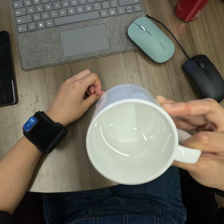
\includegraphics[width=0.66cm]{ego_anchor}};
\begin{scope}[shift={(8.70,1.72)}]
  \headtop{0.29}{eeglight}{eeglight}
  \fill[latred, opacity=0.55] (-0.12,0.02) circle (0.076);
\end{scope}
\draw[fill=bilight,  draw=bislate, line width=0.55pt] (9.20,1.72) rectangle ++(0.44,0.19);
\draw[fill=latlight, draw=latred,  line width=0.55pt] (9.20,1.53) rectangle ++(0.44,0.19);
\draw[-{Stealth[length=1.2mm,width=0.95mm]}, latred, line width=0.55pt]
      (9.28,1.625) -- (9.56,1.625);
\node[lbl, anchor=north] at (7.85,1.36) {$\mathbf{I}_t$};
\node[lbl, anchor=north] at (8.70,1.36) {$\mathbf{Z}$};
\node[lbl, anchor=north] at (9.42,1.36) {$\mathbf{H}$};

\draw[{Stealth[length=1.7mm,width=1.25mm]}-{Stealth[length=1.7mm,width=1.25mm]},
      inkgray!70, line width=0.75pt] (9.92,1.72) -- (10.34,1.72);

% --- mirrored: only the lateral half turns round ---
\node[shot] at (10.90,1.72) {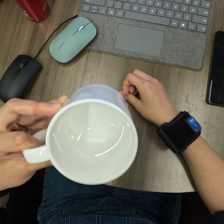
\includegraphics[width=0.66cm]{ego_anchor_flip}};
\begin{scope}[shift={(11.75,1.72)}]
  \headtop{0.29}{eeglight}{eeglight}
  \fill[latred, opacity=0.55] (0.12,0.02) circle (0.076);
\end{scope}
\draw[fill=bilight,  draw=bislate, line width=0.55pt] (12.25,1.72) rectangle ++(0.44,0.19);
\draw[fill=latlight, draw=latred,  line width=0.55pt] (12.25,1.53) rectangle ++(0.44,0.19);
\draw[-{Stealth[length=1.2mm,width=0.95mm]}, latred, line width=0.55pt]
      (12.61,1.625) -- (12.33,1.625);
\node[lbl, anchor=north, align=center] at (10.90,1.36) {mirrored\\$\mathbf{I}_t$};
\node[lbl, anchor=north] at (11.75,1.36) {$\mathcal{P}(\mathbf{Z})$};
\node[lbl, anchor=north] at (12.47,1.36) {$\mathbf{H}$};

\end{scope}

\end{tikzpicture}
